\section{Projekt robota}
\subsection{Założenia projektowe}
Wykonany robot powinien być jak najmniejszy i najprostszy w wykonaniu oraz sterowaniu tak aby móc przetesotwać przy jego pomocy działanie algorytmu A*. 
Robot będzie zbudowany z platformy, do której zostaną przyczepiony napęd, elektronika sterująca oraz bateria. 
Do platformy zostaną przymocowane dwa gotowe moduły napędowe składające się z silnika, przekładni oraz dużego koła. 
Aby pojazd stał stabilnie, doczepione zostanie trzecie koło obracające się swobodnie w każdym kierunku.
Całość będzie sterowana przy pomocy mikrokontrolera ESP32 oraz dwukanałowym sterownikiem silników DC opartym na układzie L298n.
Za zasilanie będzie odpowiadała litowo-jonowy akumulator 4S.

\subsection{Projektowanie zarysu robota w środowisku CAD}
Zbudowany ma być prosty w budowie i wykonaniu a więc założyłem że podstawa utrzymujące pozostałe komponenty
zostanie wydrukowana na drukarce 3D. Model platformy i pozostałych posiadanych elementów został wykonany w programie Fusion 360.
Modele modułów napędowych, przedniego kółka oraz baterii pozwoliły na optymalne wyznaczenie pod względem wielkości lokalizacji wszystkich elementów.

% TODO: uprościć schematy z kicada

\begin{figure}[H]
	\centering
	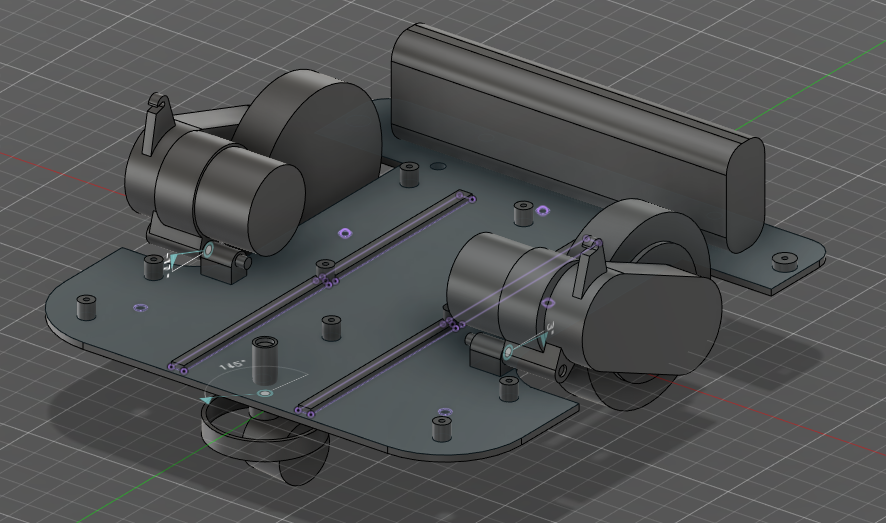
\includegraphics[width=10cm]{pages/robot/zdjecia/robotModelCaly.png}
	\caption{Zaprojektowane podwozie robota w programie Fusion360}
	\label{fig:Rys}
\end{figure}

\begin{figure}[H]
	\centering
	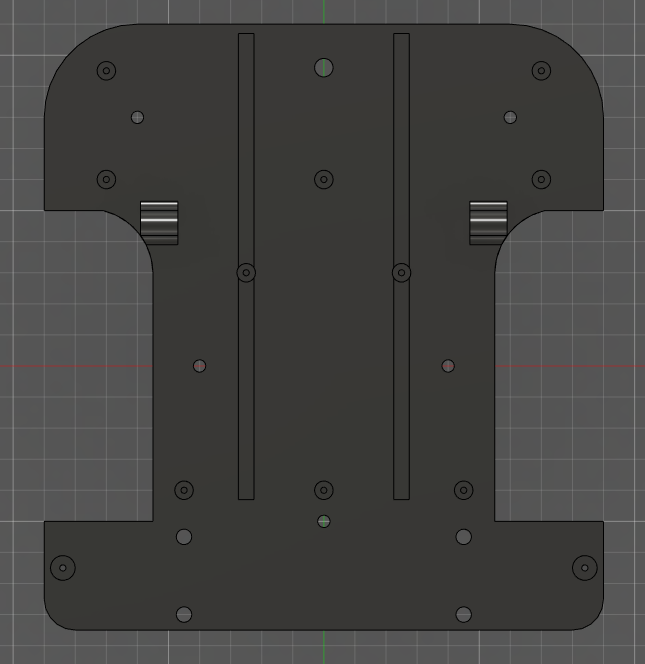
\includegraphics[width=10cm]{pages/robot/zdjecia/robotModelRama.png}
	\caption{Widok z góry na podwozie robota}
	\label{Fig:Rysunek}
\end{figure}
Model został przygotowany do druku w programie Ultimaker Cura. Parametry druku zostały dobrane 
eksperymentalnie na podstawie własnych doświadczeń. 
Podstawę wydrukowano z PLA w temperaturze 220*C i wysokości warstwy 0,2mm. 
Żeby zwiększyć wytrzymałość temperatura głowicy została lekko zawyżona względem wymagań producenta filamentu
\begin{figure}[H]
	\centering
	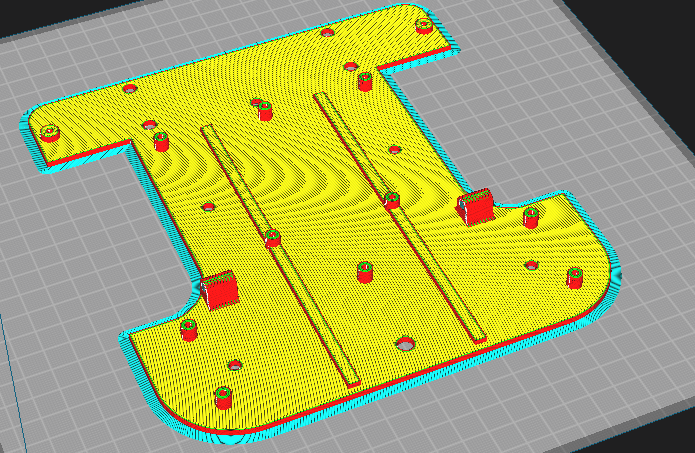
\includegraphics[width=13cm]{pages/robot/zdjecia/robotRamaCura.png}
	\caption{Widok przygotowanego do druku modelu}
	\label{fig:Rysunek}
\end{figure}
\subsection{Projekt, wykonanie oraz podłączenie elektroniki robota}
Ze względu na chęć bezprzowodowego sterowania robotem zostanie wykorzystany moduł ESP32, dla którego zostanie przygotowana odpowiednia płytka 
z wyprowadzeniami do enkoderów silnika oraz ich sterownika. Schemat elektroniczny i projekt pcb został wykonany w programie KiCad. 
\begin{figure}[H]
	\centering
	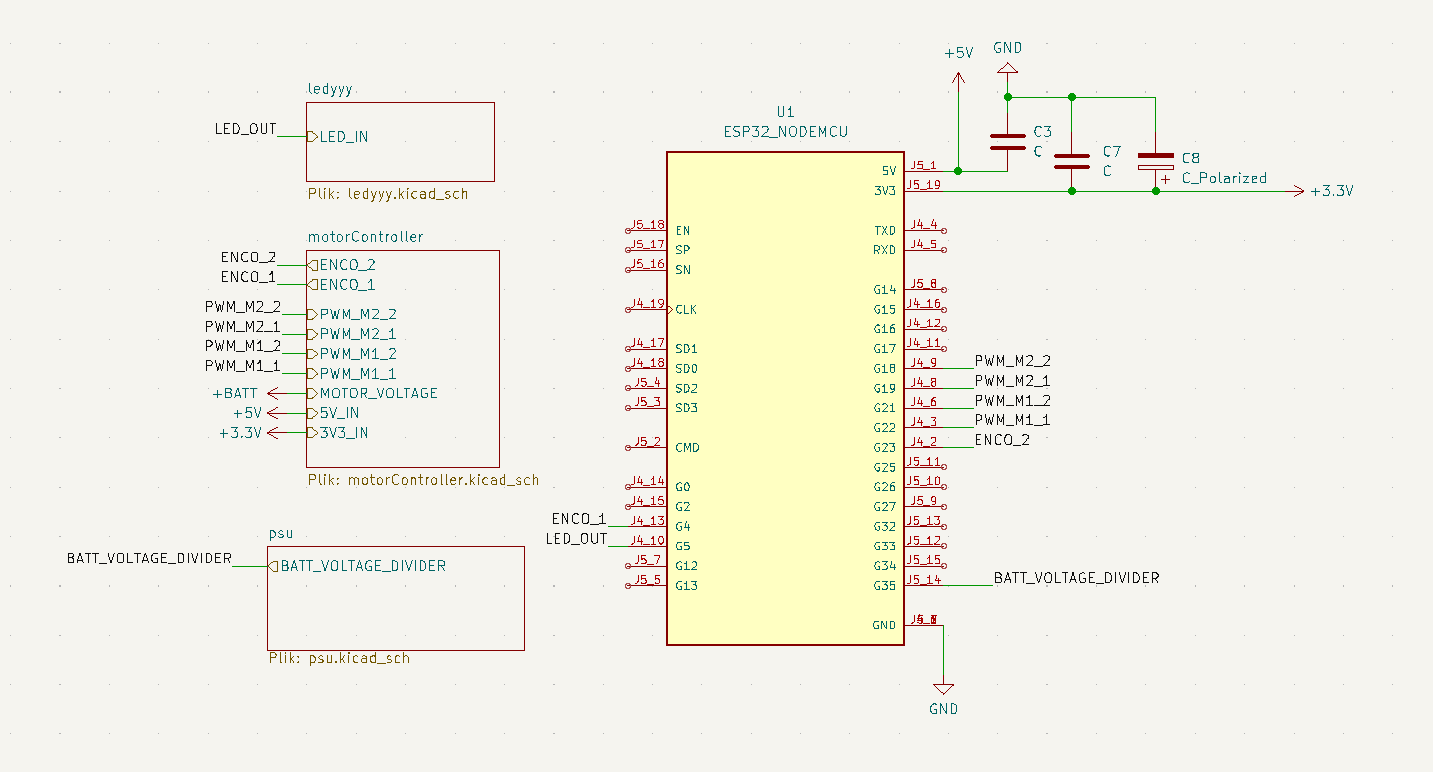
\includegraphics[width=13cm]{pages/robot/zdjecia/kicad/schematCaly.png}
	\caption{Ogólny schemat połączeń}
	\label{Fig:Rysunek}
\end{figure}
Wszystkie potrzebne elementy podsystemy mikrokontrolera zostały już wlutowane w module deweloperskim
a więc mój schemat zawiera jedynie odpowiednia połączenia z modułami roboczymi.
\begin{figure}[H]
	\centering
	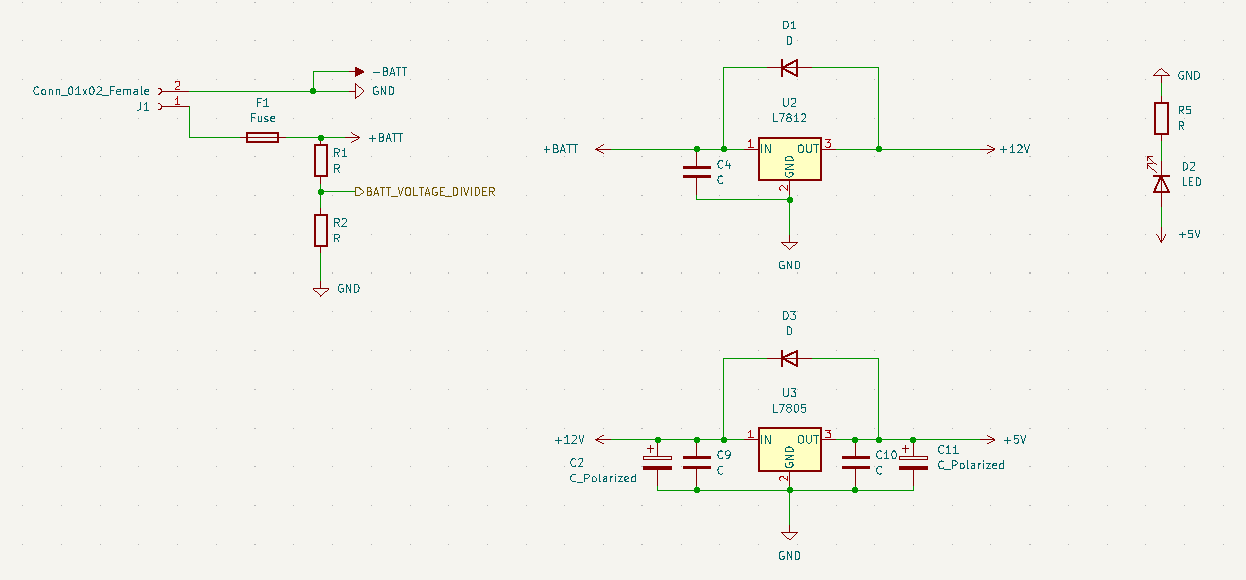
\includegraphics[width=10cm]{pages/robot/zdjecia/kicad/schematZasilanie.png}
	\caption{Ogólny schemat połączeń}
	\label{Fig:Rysunek}
\end{figure}
Użyta bateria posiada napięcie maksymalne 16,8V a więc musi zostać odpowiednio zmniejszone przed podaniem go na piny zasilania. 
Ze względu na wykorzystywaną łączność bezprzewodową a więc zwiększone zużycie prądu zmniejszanie napięcia zostało podzielone na dwie sekcje. 
Najpierw zmniejszane jest poprzez stabilizator LM7812 z 16.8V do 12V a następnie poprzez LM7805 z 12V napięcie redukowane jest do 5V. 
ESP32 zasilane jest napięciem 3.3V tworzonym poprzez stabilizator AMS1117 w module deweloperskim. 
Aby zredukować spadki napięć powstałe przy nagłym poborze prądu dodałem dodatkowe kondensatory filtrujące. 
Dodatkowo na schemacie widoczny jest dzielnik napięcia pozwalający na poziom naładowania baterii przez sterownik 
jednak ostatecznie nie został on wykorzystany w projekcie.
\begin{figure}[H]
	\centering
	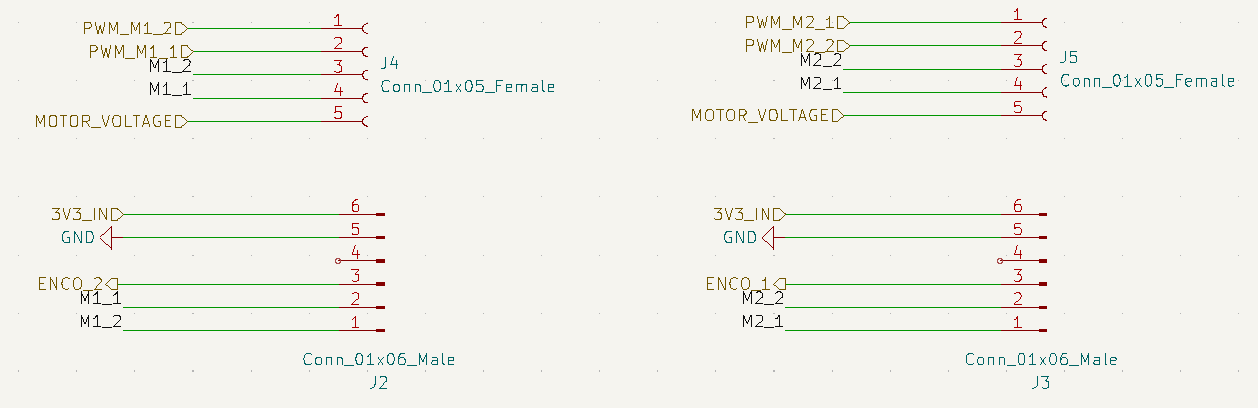
\includegraphics[width=16cm]{pages/robot/zdjecia/kicad/schematSilniki.png}
	\caption{Ogólny schemat połączeń silników}
	\label{Fig:Rysunek}
\end{figure}
Użyte moduły napędowe posiadają enkoder inkrementalny zbudowany z czujnika halla i tarczy magnetycznej zamocowanej na wale silnika.
Czujnik halla jest zasilany napięciem 3.3V i na wyjściu otrzymujemy sygnał ze "szpilkami" proporcjonalny do aktualnych obrotów silnika. 
Silniki zasilane są poprzez moduł z układem L298n a prędkość ustalana jest poprzez odpowiednio generowany sygnał PWM. 
\begin{figure}[H]
	\centering
	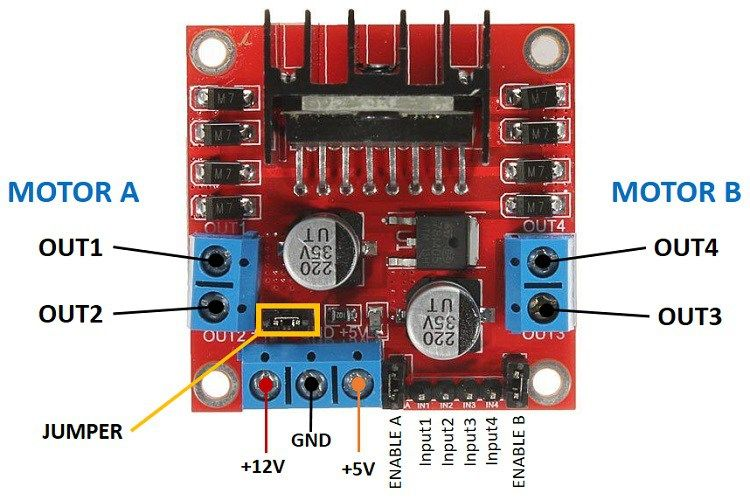
\includegraphics[width=10cm]{pages/robot/zdjecia/l298n_modul.jpg}
	\caption{Wykorzystany moduł do sterowania silnikami, L298n}
	\label{Fig:Rysunek}
\end{figure}
\begin{figure}[H]
	\centering
	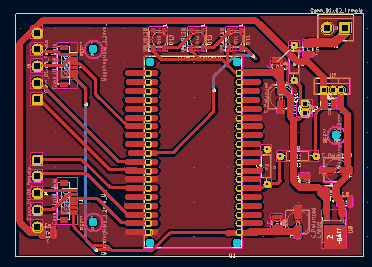
\includegraphics[width=6cm]{pages/robot/zdjecia/kicad/kiCad_PCB.png}
	\caption{Projekt PCB}
	\label{Fig:Rysunek}
\end{figure}
Na widocznym powyżej zdjęciu widać ostateczną wersje projektu pcb. 
Można zauważyć że widoczne są na niej trzy adresowalne diody świecące, które nie zostały wykorzystywane przez napisane oprogramowanie.


\subsection{Oprogramowanie robota}

Program sterujący robotem został napisany w C++. 
Szkielet aplikacji bazuje na projekcie utworzonym przez framework IDF w wersji 4.4 udostępnionym 
przez producenta użytego procesora. Po za tym użyta została biblioteka implementująca 
system czasu rzeczywistego FreeRTOS i ASIO do obsługi połączenia TCP. 
\begin{figure}[H]
	\centering
	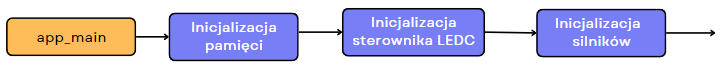
\includegraphics[width=14cm]{pages/robot/zdjecia/schematy/softSchematCz1.png}
	\caption{Schemat programu cz.1 }
	\label{Fig:Rysunek}
\end{figure}
\begin{figure}[H]
	\centering
	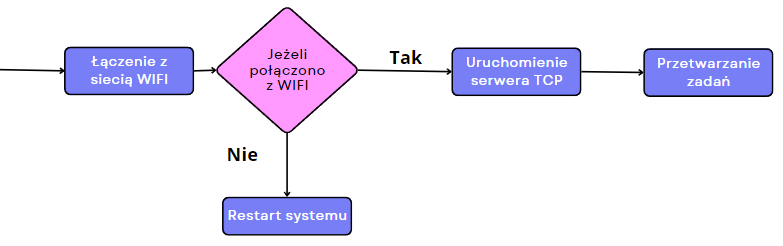
\includegraphics[width=14cm]{pages/robot/zdjecia/schematy/softSchematCz2.png}
	\caption{Schemat programu cz.2}
	\label{Fig:Rysunek}
\end{figure}

Działanie programu rozpoczyna się od wywołania funkcji app\_main, inicjalizacji funkcji systemowych i sterowników silników.
W dalszej kolejności nawiązywana jest łączność z siecią WiFi. W przypadku braku połączenia system resetuje się. 
Po poprawnym połączeniu uruchamiany jest kontekst biblioteki ASIO a następnie uruchomienie serwera TCP.
Klienci połączeniu do serwera utowrzonego przez robota wysyłają komendy tekstowe wraz z odpowiednimi arguemntami, które
robot odpowiednio przetwarza. 
\subsubsection{Sterowanie silnikami}
Sterowanie silnikami odbywa się poprzez klasę MotorController, która dziedziczy po klasie PIDController implementującej regulator PID.
Obiekt automatycznie tworzy timer uruchamiający co 100ms metodę aktualizującą wyjścia sterujące silnikiem. 
Aktualna prędkość wyznaczana jest na podstawie przerwania wyzwalanego przez enkoder silnika. Przerwanie inkrementuje licznik, 
czyszczony przez wcześniej opisany timer. Nastawy regulatora PID zostały dobrane eksperymentalinie, człon proporcjonalny wynosi 8 a całkujący i różniczkujący 0,1. 


% TODO: opis regulatora PID, wzory itp
\subsubsection{Serwer TCP}

%TODO: opis serwera TCP
